%%%%%%%%%%%%%%%%%%%%%%%%%%%%%%%%%%%%%%%%%%%%%%%%%%%%%%%%%%%%%%%%%%%%%%%%%%%%%%%
%%                                                                           %%
%%                             Trabajo indito                               %%
%%                                                                           %%
%%%%%%%%%%%%%%%%%%%%%%%%%%%%%%%%%%%%%%%%%%%%%%%%%%%%%%%%%%%%%%%%%%%%%%%%%%%%%%%

\cabecera{cap:popstruc}
                 {Population structure as a complex network}
\chapter{\textit{Population structure as a complex network}}
\label{cap:popstruc}
\cabecera{cap:trabajo}
                 {Population structure as a complex network}

%%%%%%%%%%%%%%%%%%%%%%%%%%%%%%%%%%%%%%%%%%%%%%%%%%%%%%%%%%%%%%%%%%%%%%%%%%%%%%%

%\vfill
%\itshape
%En los problemas de clasificacin de patrones se busca minimizar el nmero de patrones mal clasificados (el error), sin embargo, en muchas aplicaciones reales hay que tener en cuenta por separado el error tipo I (falsos positivos) y el error tipo II (falsos negativos).
%Suele ser un problema complejo ya que un intento de minimizar uno de ellos, hace que el otro crezca.
%Es ms, en ocasiones uno de estos tipos de error puede ser ms importante que el otro, y se debe buscar un compromiso que minimice el ms importante de los dos.
%La medida estadstica ms utilizada, significancia estadstica, es una medida del error tipo I. Sin embargo, no ofrece garantas sobre el tipo II.

%A pesar de la importancia de los errores tipo II, la mayora de los mtodos de clasificacin slo tienen en cuenta el error de clasificacin global.
%En este trabajo se propone la optimizacin de ambos tipos de error de clasificacin utilizando un algoritmo multiobjetivo en el que cada tipo de error y el tamao de red son objetivos de la funcin de evaluacin (fitness).

%Se ha utilizado una versin modificada del mtodo G-Prop (diseo y optimizacin de perceptrones multicapa usando un algoritmo evolutivo) para optimizar simultneamente la estructura de la red neuronal y los errores tipo I y II.

%Debido a la carga computacional que supone la ejecucin de un algoritmo evolutivo para el diseo de redes neuronales, se propone la paralelizacin utilizando el modelo isla como forma de distribuir la carga en una red heterognea.
%\upshape
%\clearpage

%%%%%%%%%%%%%%%%%%%%%%%%%%%%%%%%%%%%%%%%%%%%%%%%%%%%%%%%%%%%%%%%%%%%%%%%%%%%%%%

%%%%%%%%%%%%%%%%%%%%%%%%%%%%%%%%%%%%%%%%%%%%%%%%%%%%%%%%%%%%%

To help understand the role of the population structure in a P2P EA, we introduce the structural design of a simple and easy understandable complex network proposed by Watts and Strogatz in \cite{wattsstrogatz}. As described by the authors, the procedure for building a small-world topology can start from a ring lattice with $n$ vertices and $k$ edges per vertex. With a given probability $p$, each edge is rewired at random. This way for a rewiring factor of
$p=0$ the ring lattice is kept while for $p=1$ a random graph is generated. It is within the intermediate values of $p$ where the graph gets small-world structure.


%\begin{figure}[t]
%\begin{center}
%\includegraphics[width=\textwidth]{lineaInv}
%\end{center}
%\vspace{-2ex}
%\caption{Esquema de capas de la línea de investigación}
%\label{fig:lineaInv}
%\end{figure}

\begin{figure}[htbp]
\begin{center}
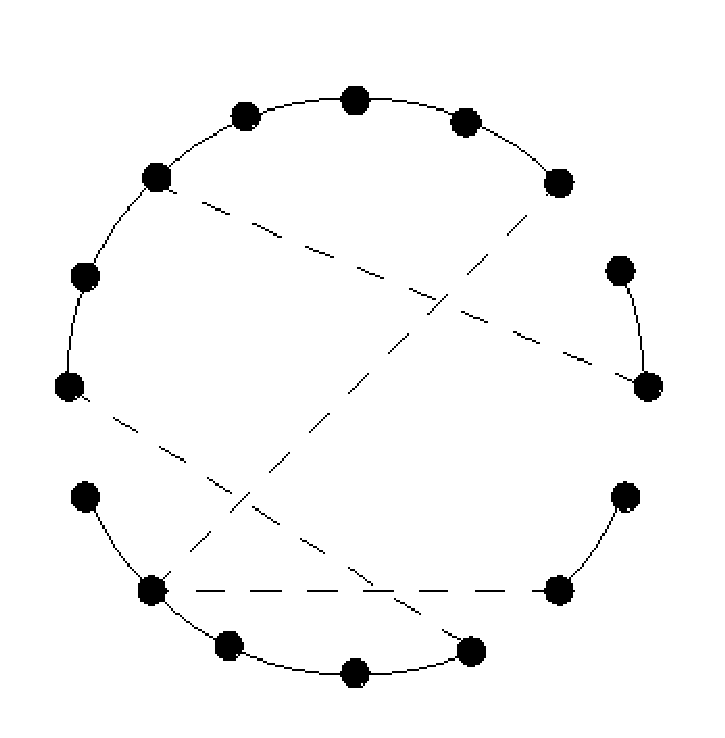
\includegraphics[width=\textwidth/3]{smallworld}
\end{center}
\vspace{-2ex}
\caption{Small-world graph built from a ring lattice with $n=16$, $k=2$ and $p=0.2$.}
\label{fig:small-world}
\end{figure}


In Figure \ref{fig:small-world}, the edges have been rewired with a probability of $p=0.2$ ({\em dashed lines}). Being the {\sf Characteristic Path Length (CPL)} the average shortest distance between any pair of nodes, this graph has $CPL=3.7$, the original ring lattice had $CPL=4.26$ while a complete graph (i.e. panmictic) would have $CPL=1.0$. Such a characteristic is related to the selection pressure within an structured EA, the smaller the $CPL$ the stronger the selection pressure is.

Takeover time curves are good descriptors on the way that the population structure and the selection method affect the environmental selection pressure. Tomassini in \cite{tomassini} defines the takeover time as the time that takes for a single, best individual to take over the entire population without any other mechanism than selection. Hence, takeover time is the proportion of best individuals as a function of time. 


\begin{figure}[htbp]
\begin{center}
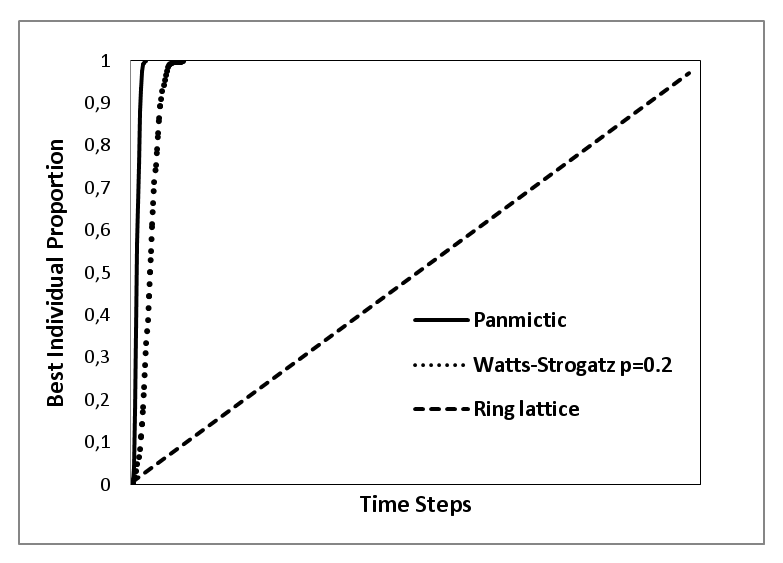
\includegraphics[width=\textwidth/2]{takeoverwattsstrogatz}
\end{center}
\vspace{-2ex}
\caption{Takeover time curves in a panmictic graph, Watts-Strogatz graph with $p=0.2$ and the original ring lattice with $k=2$. Results for $n=1000$ and binary tournament. }
\label{fig:takeoversw}
\end{figure}



Topologies with a smaller CPL imply a shorter takeover time curve, consequently, a higher selection pressure and a more exploitative behaviour. Figure \ref{fig:takeoversw} shows that the selection pressure in a panmictic graph is much higher than in a ring lattice while a small-world graph keeps intermediate values. Keeping the selection pressure well balanced is of the maximum interest in order to find a good compromise between the explorative and exploitative components of an EA. As the topology shown above, P2P topologies offer intermediate levels of environmental selection pressure when used as population structure of an EA.
